     %%%%%%%%%%%%%%%%%%%%
     %                                                   %
     %  capitolo1.tex   %
     %                  %
     %%%%%%%%%%%%%%%%%%%%

\section{Esperimenti}\label{sec:esperimenti}

Il software prodotto è stato testato su molteplici video, tra i quali ne sono stati selezionati tre che si distinguevano per le condizioni di esecuzione, in particolare stimolando caratteristiche specifiche dei due algoritmi di tracking, in modo da efatizzarne i risultati. I tre filmati sono caratterizzati da una ripresa a camera fissa, con un singolo oggetto in movimento che può sia uscire dall'inquadratura che nascondersi dietro qualche ostacolo all'interno della scena (occlusione). 

In ognuno dei tre filmati i primi frames sono di solo sfondo, ovvero non compare alcun oggetto in moto; questa scelta è stata effettuata per facilitare l'applicazione del Background Subtraction.\\

Per ciascun video abbiamo osservato/confrontato il comportamento dei due filtri al variare di alcuni parametri quali:
\begin{itemize}
\item frequenza di campionamento (MOD)
\item covarianza relativa al rumore del processo studiato (Q) (stabilisce la tolleranza consentita alla predizione del filtro di Kalman)
\item numero di campioni utilizzati dal Condensation\\
\end{itemize}

I risultati prodotti per ciascuna prova sono rappresentati in due grafici:
\begin{itemize}
\item Il primo rappresenta per ogni campionamento:
\begin{itemize}
\item la posizione dell'oggetto
\item la posizione predetta dal filtro di Kalman
\item la posizione predetta dal Condensation
\end{itemize}
\item Il secondo rappresenta per ogni campionamento di quanto rispettivamente ciascuna predizione si discosta dalla posizione reale dell'oggetto.
\end{itemize}

Inoltre per ogni test viene dato il valore medio della distanza (in pixels) tra posizione predetta e posizione reale, sia per il filtro di Kalman \begin{math}(\bar \delta_K)\end{math} che per il Condensation \begin{math}(\bar \delta_C)\end{math}, oltre al valore della varianza media per il Condensation \begin{math}(\sigma_x,\sigma_y)\end{math}.


\newpage

\subsection{Video: movies12.mjpeg}\label{sec:video-occ}
\begin{itemize}
\item risoluzione: 640x480
\item fps: 25.00
\item durata: 50.4 s
\end{itemize}

\begin{figure}[hb]
\centering
	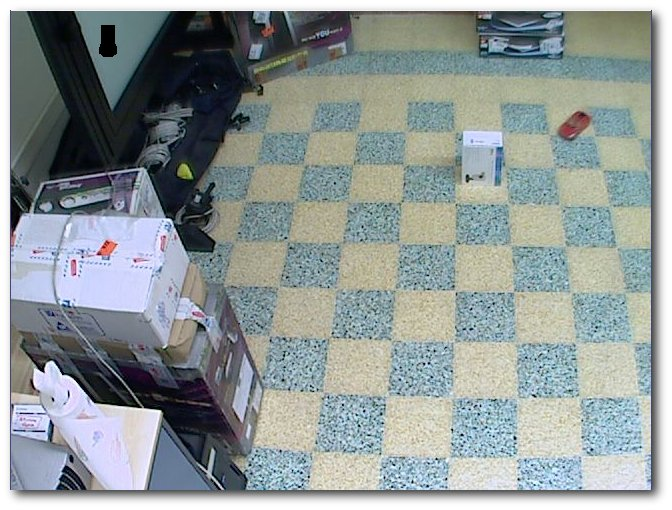
\includegraphics[scale=0.5]{movie12.jpg}
\caption{\textit{movie12 screenshot}}
\end{figure}

Si tratta di una ripresa trasversale dall'alto di un automobilina radiocomandata. In questa scena i punti di occlusione sono due: una scatola al centro della scena e un ostacolo sulla sinistra. La macchina non subisce repentine accelerazioni o decelerazioni, in generale ruota attorno alla scatola centrale e riamane nascosta dietro questa per un po'. L'automobilina non esce mai dalla scena.

%\begin{figure}[hb]
%\centering%
%	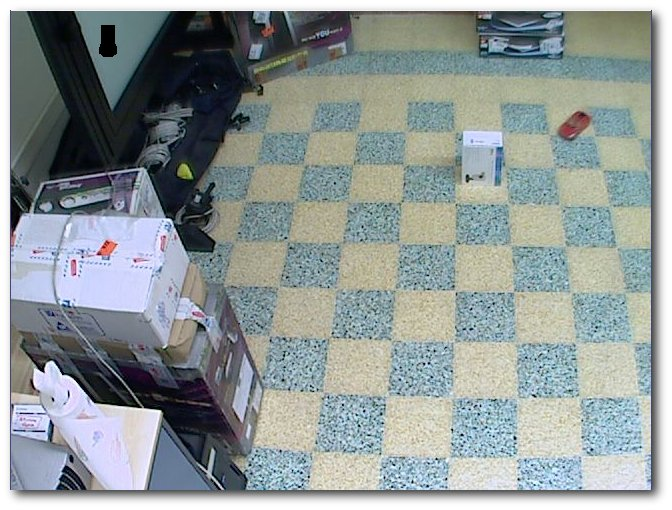
\includegraphics[scale=0.5]{movie12.jpg}
%\caption{\textit{movie12 screenshot}}
%\end{figure}
 
\newpage
\subsubsection{Test 1: MOD=3 , Q=1000, S=1000}

\begin{figure}[hb]
\centering
	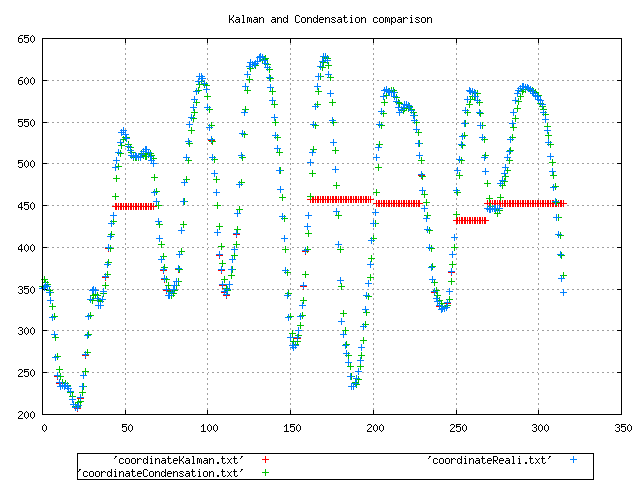
\includegraphics[scale=0.4]{../../esperimenti/movie12/mod_3-Q_1000-S_1000/plot.png}
\caption{\textit{Test 1: Tracciamento}}
\end{figure}

\begin{figure}[hb]
\centering
	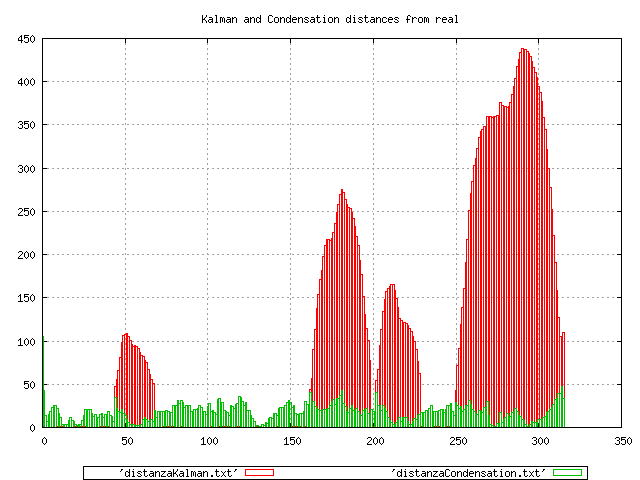
\includegraphics[scale=0.4]{../../esperimenti/movie12/mod_3-Q_1000-S_1000/plot-distances.png}
\caption{\textit{Test 1: Previsioni}}
\end{figure}

Statistiche:
\begin{itemize}
\item \begin{math} \bar \delta_K: 105 \end{math}
\item \begin{math} \bar \delta_C: 18 \end{math}
\item \begin{math}(\sigma_x,\sigma_y)\end{math}: (112,81)
\end{itemize}

Appare evidente che con queste impostazioni il filtro di Kalman non è in grado di mantenere traccia correttamente dell'oggetto, poichè più di una misurazione è persa a causa dell'occlusione. L'area di tolleranza per Kalman non è sufficiente. Tuttavia non appena l'oggetto ripassa vicino a dove Kalman si è fermato, questo ricomincia ad essere tracciato correttamente. Differentemente il Condenstaion non perde mai l'oggetto, ma la stima del moto è decisamente meno precisa.

\newpage

\subsubsection{Test 2: MOD=3, Q=2000, S=1000}

\begin{figure}[hb]
\centering
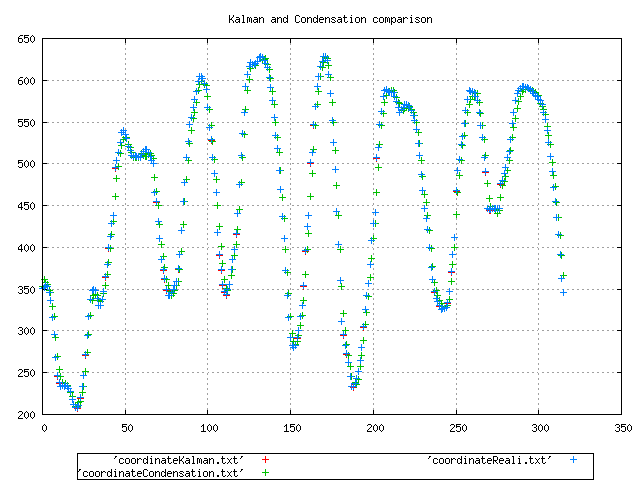
\includegraphics[scale=0.4]{../../esperimenti/movie12/mod_3-Q_2000-S_1000/plot.png}
\caption{\textit{Test 2: Tracciamento}}
\end{figure}

\begin{figure}[hb]
\centering
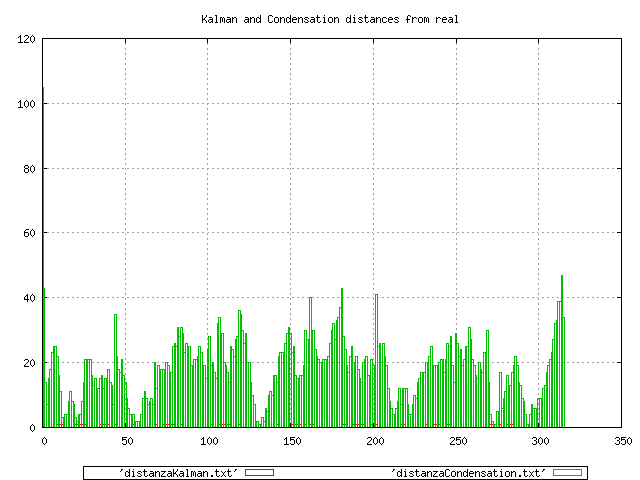
\includegraphics[scale=0.4]{../../esperimenti/movie12/mod_3-Q_2000-S_1000/plot-distances.png}
\caption{\textit{Test 2: Previsioni}}
\end{figure}

Statistiche:
\begin{itemize}
\item \begin{math} \bar \delta_K: 0 \end{math}
\item \begin{math} \bar \delta_C: 18 \end{math}
\item \begin{math}(\sigma_x,\sigma_y)\end{math}: (112,81)
\end{itemize}

Allargando l'area di confidenza per Kalman l'oggetto non viene mai perso e il tracciamento risulta pressochè perfetto. Il comportamrento in questo caso è evidentemente migliore del Condesation. Purtroppo un'area di confidenza troppo ampia potrebbe in alcune circostanze far perdere di validità al tracciamento. 

\newpage
\subsubsection{Test 3: MOD=3, Q=1000, S=5000}

\begin{figure}[hb]
\centering
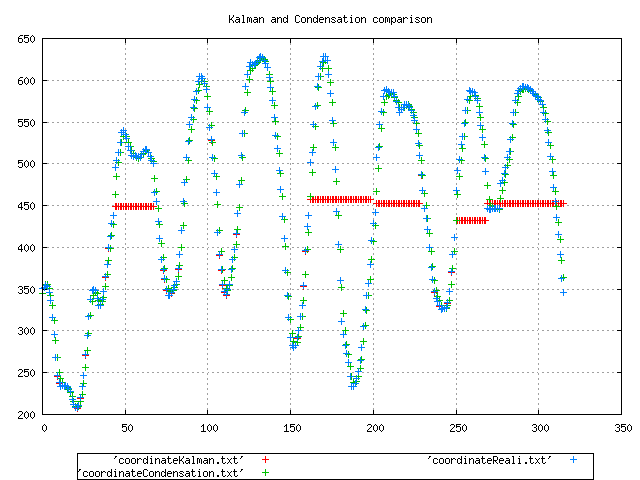
\includegraphics[scale=0.4]{../../esperimenti/movie12/mod_3-Q_1000-S_5000/plot.png}
\caption{\textit{Test 3: Tracciamento}}
\end{figure}

\begin{figure}[hb]
\centering
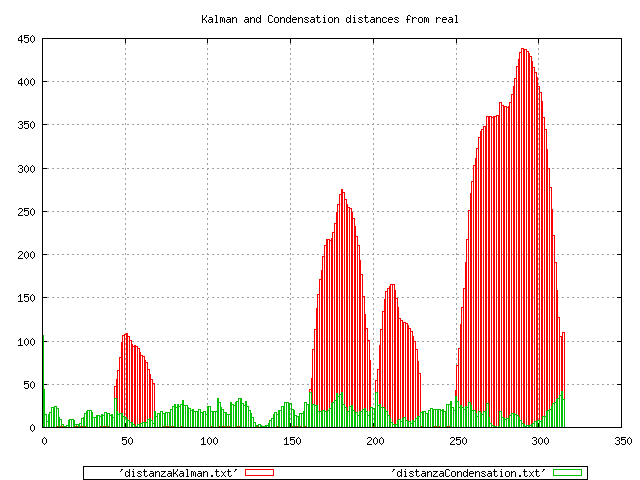
\includegraphics[scale=0.4]{../../esperimenti/movie12/mod_3-Q_1000-S_5000/plot-distances.png}
\caption{\textit{Test 3: Previsioni}}
\end{figure}

Statistiche:
\begin{itemize}
\item \begin{math} \bar \delta_K: 105 \end{math}
\item \begin{math} \bar \delta_C: 17 \end{math}
\item \begin{math}(\sigma_x,\sigma_y)\end{math}: (109,81)
\end{itemize}

Con questo test cominciamo a verificare il comportamento del Condensation alla variazione del numero di samples.
E' immediato osservare come aumentando il numero di samples da 1000 a 5000 questo non porti in media nessun significativo miglioramento.

\newpage
\subsubsection{Test 4: MOD=3, Q=1000, S=100}

\begin{figure}[hb]
\centering
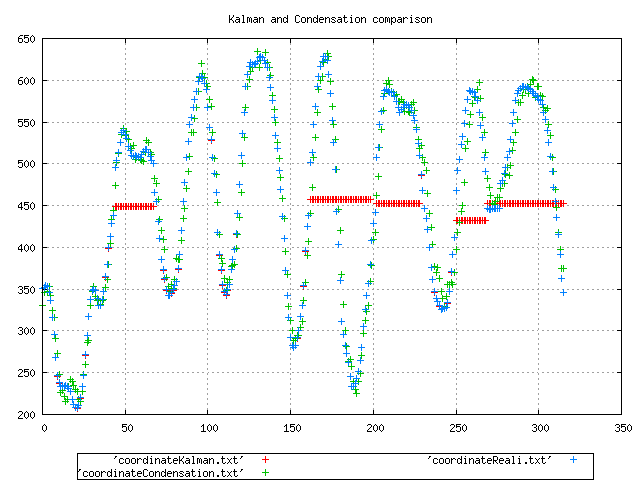
\includegraphics[scale=0.4]{../../esperimenti/movie12/mod_3-Q_1000-S_100/plot.png}
\caption{\textit{Test 4: Tracciamento}}
\end{figure}

\begin{figure}[hb]
\centering
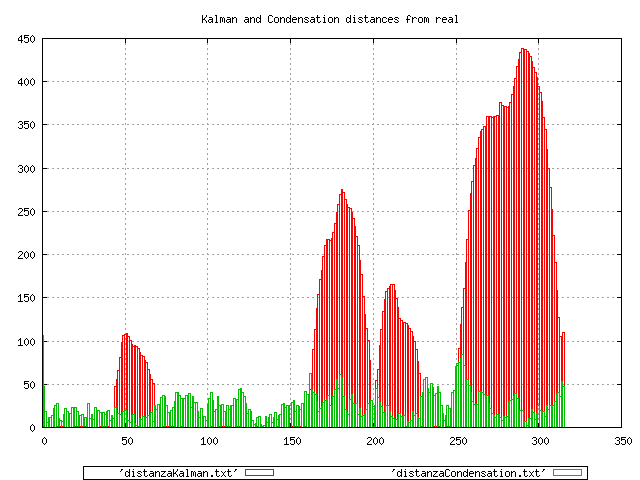
\includegraphics[scale=0.4]{../../esperimenti/movie12/mod_3-Q_1000-S_100/plot-distances.png}
\caption{\textit{Test 4: Previsioni}}
\end{figure}

Statistiche:
\begin{itemize}
\item \begin{math} \bar \delta_K: 105 \end{math}
\item \begin{math} \bar \delta_C: 24 \end{math}
\item \begin{math}(\sigma_x,\sigma_y)\end{math}: (140,92)
\end{itemize}


Di contro con questo test si nota come passando da 1000 a 100 samples invece il risultato sia notevolemente diverso. La stima del moto come si vede dal grafico è notevolemente peggiore nel secondo caso. 
Fortunatamente ha anche poco senso limitare così tanto il numero di samples, mentre un numero molto alto di samples per noi non comporta nessun particolare svantaggio. 

\newpage
\subsubsection{Test 5: MOD=3, Q=1000, S=10}

\begin{figure}[hb]
\centering
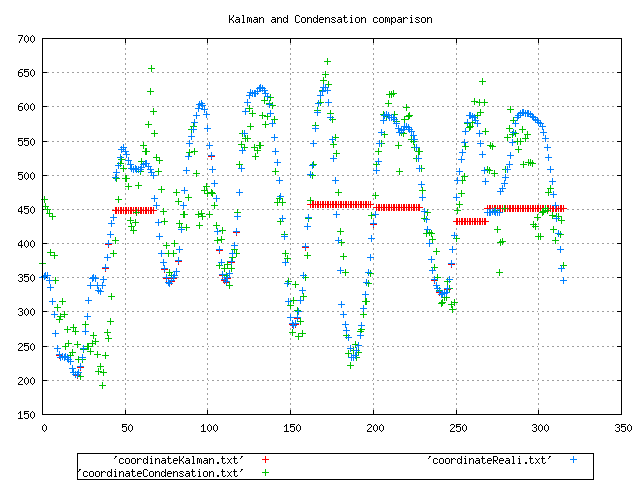
\includegraphics[scale=0.4]{../../esperimenti/movie12/mod_3-Q_1000-S_10/plot.png}
\caption{\textit{Test 5: Tracciamento}}
\end{figure}

\begin{figure}[hb]
\centering
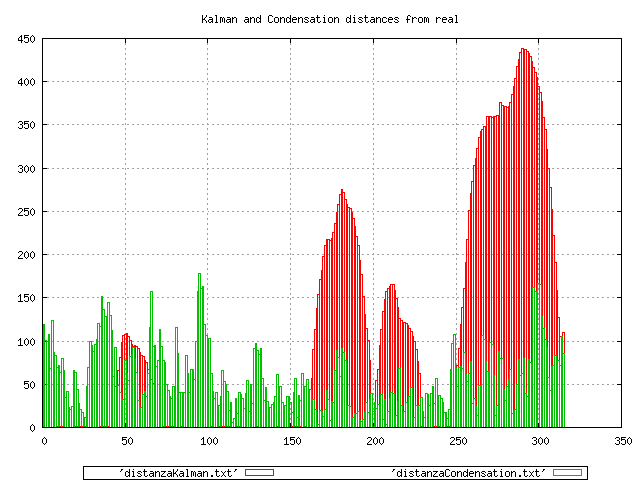
\includegraphics[scale=0.4]{../../esperimenti/movie12/mod_3-Q_1000-S_10/plot-distances.png}
\caption{\textit{Test 5: Previsioni}}
\end{figure}

Statistiche:
\begin{itemize}
\item \begin{math} \bar \delta_K: 105 \end{math}
\item \begin{math} \bar \delta_C: 55 \end{math}
\item \begin{math}(\sigma_x,\sigma_y)\end{math}: (195,112)
\end{itemize}


Abbiamo proseguito nel diminuire il numero di Samples per il Condensation passando a 10, il confronto tra il caso in cui i samples erano 1000 è autoesplicativo: il risultato è notevolemente peggiore. Come ci si poteva aspettare in condizioni estreme di lavoro le previsioni sono decisamente inattendibili.

\newpage
\subsection{Video: tappetonomod.avi}

\begin{itemize}
\item risoluzione: 320x240
\item fps: 10.00
\item durata: 60 s
\end{itemize}

Si tratta di una ripresa trasversale dall'alto. L'oggetto in movimento è un'automobilina radiocomandata che si muove su un'area delimitata da un tappeto. Il moto dell'automobilina subisce repentine accelerazioni e decelerazioni. Non ci sono oggetti occludenti, ma l'automobilina entra ed esce totalmente o parzialmente più di una volta dalla scena.

\begin{figure}[hb]
\centering
	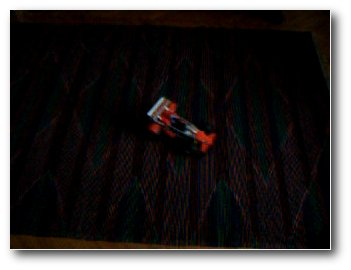
\includegraphics[scale=0.5]{tappeto_nomod.jpg}
\caption{\textit{tappeto-nomod screenshot}}
\end{figure}

\newpage
\subsubsection{Test 6: MOD=3, Q=1000, S=1000}

\begin{figure}[hb]
\centering
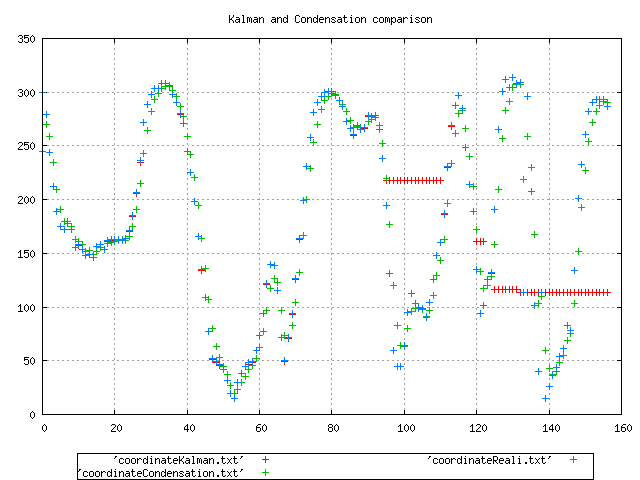
\includegraphics[scale=0.4]{../../esperimenti/tappeto_nozoom/mod_3-Q_1000-S_1000/plot.png}
\caption{\textit{Test 6: Tracciamento}}
\end{figure}

\begin{figure}[hb]
\centering
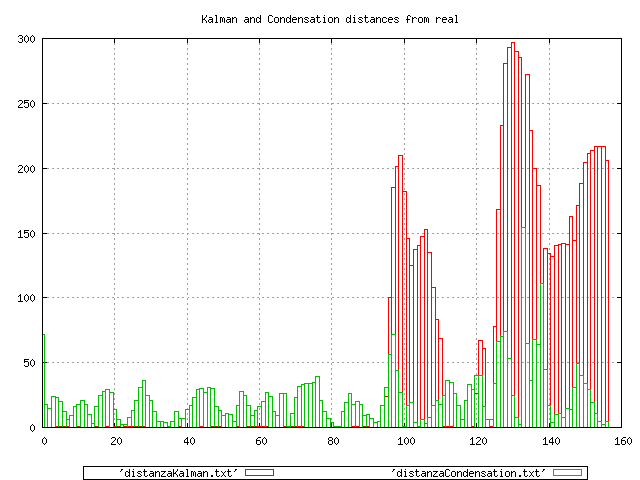
\includegraphics[scale=0.4]{../../esperimenti/tappeto_nozoom/mod_3-Q_1000-S_1000/plot-distances.png}
\caption{\textit{Test 6: Previsioni}}
\end{figure}

Statistiche:
\begin{itemize}
\item \begin{math} \bar \delta_K: 53 \end{math}
\item \begin{math} \bar \delta_C: 22 \end{math}
\item \begin{math}(\sigma_x,\sigma_y)\end{math}: (53,22)
\end{itemize}

La macchinina si sposta in modo molto rapido. Kalman si comporta in modo egregio fintanto che l'oggetto si trova nell'inquadratura e che l'accelerazione della macchina non è tale da far uscire l'oggetto dall'area di previsione. Il Condensation mantiene un buon comportamento anche se mai perfetto.

\newpage
\subsubsection{Test 7: MOD=5, Q=1000, S=1000}

\begin{figure}[hb]
\centering
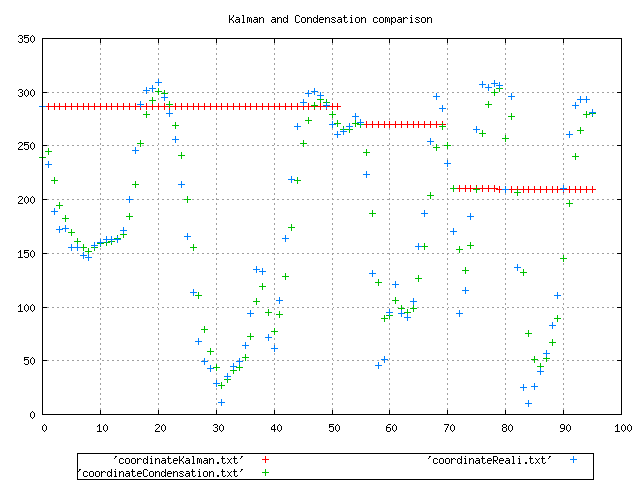
\includegraphics[scale=0.4]{../../esperimenti/tappeto_nozoom/mod_5-Q_1000-S_1000/plot.png}
\caption{\textit{Test 7: Tracciamento}}
\end{figure}

\begin{figure}[hb]
\centering
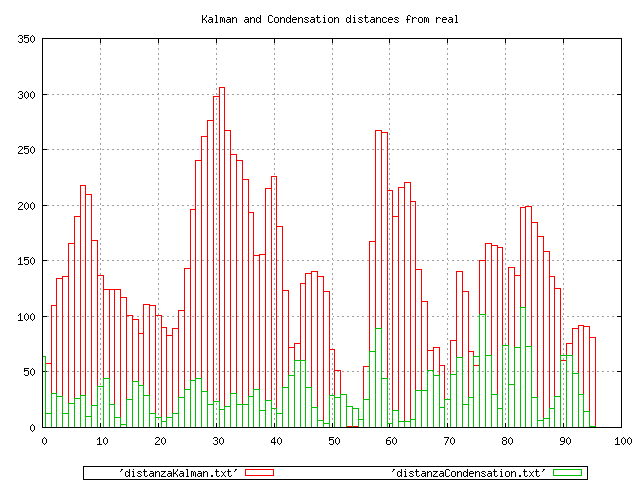
\includegraphics[scale=0.4]{../../esperimenti/tappeto_nozoom/mod_5-Q_1000-S_1000/plot-distances.png}
\caption{\textit{Test 7: Previsioni}}
\end{figure}

Statistiche:
\begin{itemize}
\item \begin{math} \bar \delta_K: 137 \end{math}
\item \begin{math} \bar \delta_C: 31\end{math}
\item \begin{math}(\sigma_x,\sigma_y)\end{math}: (56,40)
\end{itemize} 

Come prevedibile la rapidità di moto di questo oggetto mal si concilia una misurazione effettuata ad intervalli ampi. Entrambi i filtri si comportano in modo non proprio ottimale, in particolare Kalman perde quasi immediatamente l'oggetto. 

\newpage
\subsubsection{Test 8: MOD=2, Q=1000, S=1000}

\begin{figure}[hb]
\centering
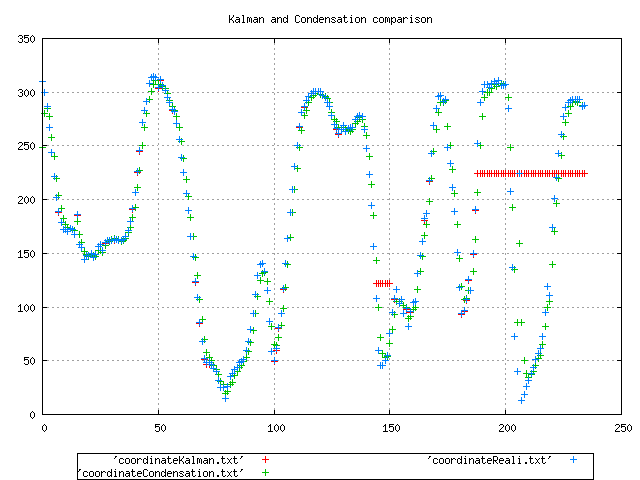
\includegraphics[scale=0.4]{../../esperimenti/tappeto_nozoom/mod_2-Q_1000-S_1000/plot.png}
\caption{\textit{Test 8: Tracciamento}}
\end{figure}

\begin{figure}[hb]
\centering
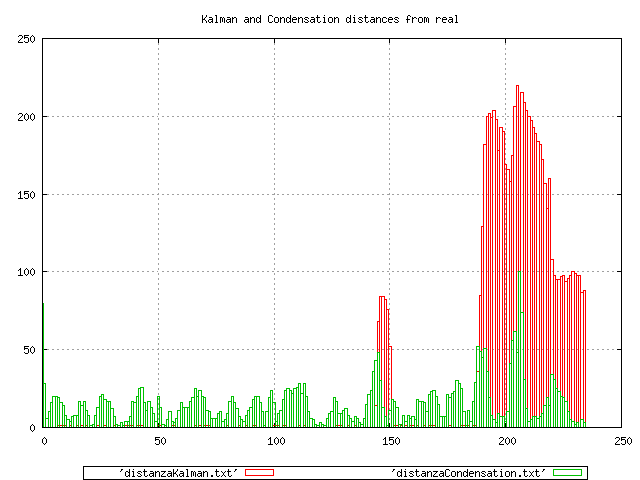
\includegraphics[scale=0.4]{../../esperimenti/tappeto_nozoom/mod_2-Q_1000-S_1000/plot-distances.png}
\caption{\textit{Test 8: Previsioni}}
\end{figure}

Statistiche:
\begin{itemize}
\item \begin{math} \bar \delta_K: 32 \end{math}
\item \begin{math} \bar \delta_C: 15 \end{math}
\item \begin{math}(\sigma_x,\sigma_y)\end{math}: (55,41)
\end{itemize}

La situazione decisamente migliora se invece campioniamo ogni 2 frames. Kalman fintato che non perde l'oggetto si comporta meglio del Condensation, in media però il Condensation risulta migliore.


\newpage
\subsubsection{Test 9: MOD=1, Q=2000, S=1000}

\begin{figure}[hb]
\centering
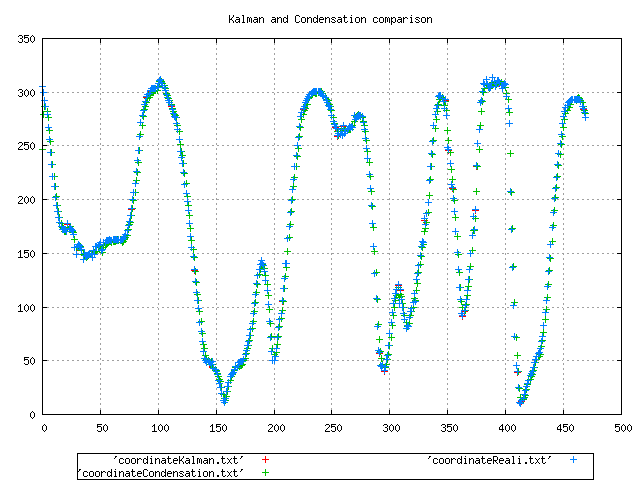
\includegraphics[scale=0.4]{../../esperimenti/tappeto_nozoom/mod_1-Q_2000-S_1000/plot.png}
\caption{\textit{Test 9: Tracciamento}}
\end{figure}

\begin{figure}[hb]
\centering
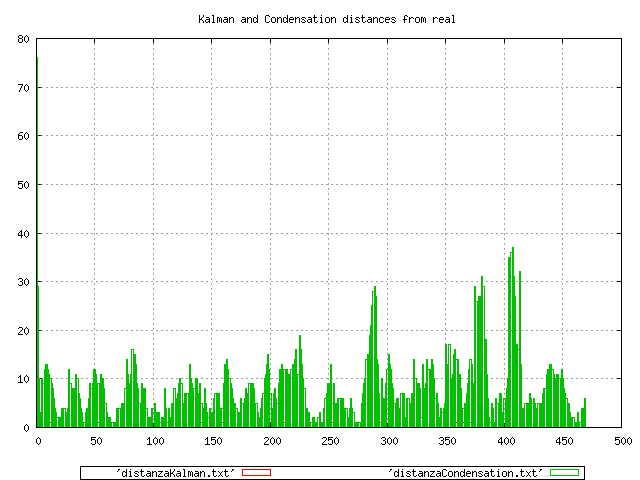
\includegraphics[scale=0.4]{../../esperimenti/tappeto_nozoom/mod_1-Q_2000-S_1000/plot-distances.png}
\caption{\textit{Test 9: Previsioni}}
\end{figure}

Statistiche:
\begin{itemize}
\item \begin{math} \bar \delta_K: 0 \end{math}
\item \begin{math} \bar \delta_C: 8 \end{math}
\item \begin{math}(\sigma_x,\sigma_y)\end{math}: (55,41)
\end{itemize}

Ingrandendo l'area di tolleranza per Kalman e prendendo la misura ogni frame Kalman traccia perfettamente il moto dell'oggetto e anche il Condensation migliora il proprio comportamento. Questa è una situazione ottimale, però decisamente poco realistica. Sono risultati che possiamo ottenere solo perchè stiamo tracciando il moto di un oggetto del quale conosciamo tutto dettagliatamente (Video Stream).

\newpage
\subsubsection{Test 10: MOD=1, Q=500, S=1000}

\begin{figure}[hb]
\centering
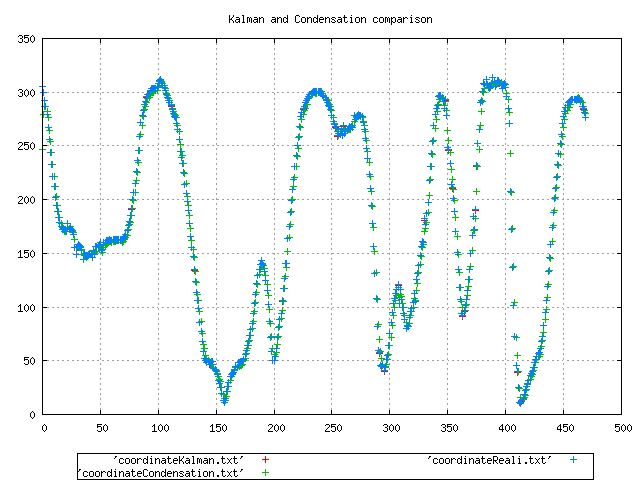
\includegraphics[scale=0.4]{../../esperimenti/tappeto_nozoom/mod_1-Q_500-S_1000/plot.png}
\caption{\textit{Test 10: Tracciamento}}
\end{figure}

\begin{figure}[hb]
\centering
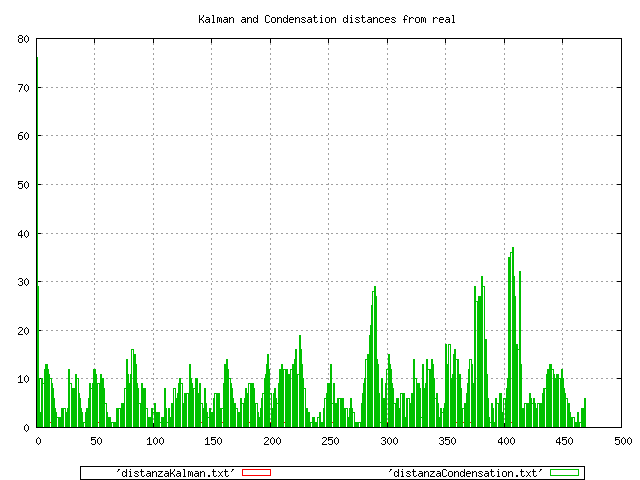
\includegraphics[scale=0.4]{../../esperimenti/tappeto_nozoom/mod_1-Q_500-S_1000/plot-distances.png}
\caption{\textit{Test 10: Previsioni}}
\end{figure}

Statistiche:
\begin{itemize}
\item \begin{math} \bar \delta_K: 0 \end{math}
\item \begin{math} \bar \delta_C: 8 \end{math}
\item \begin{math}(\sigma_x,\sigma_y)\end{math}: (55,41)
\end{itemize}

Campionando ogni frame, anche diminuendo l'area dell'ellisse di tolleranza per Kalman i risultati non cambiano.

\newpage
\subsection{Video: singlecar.avi}

\begin{itemize}
\item risoluzione: 648x484
\item fps: 30.00
\item durata: 33 s
\end{itemize}

Anche in questo caso il video è di un'automobilina radiocomadata ripresa dall'alto trasversalmente. A differenza che negli altri video non ci sono oggetti occludenti e il moto è piuttosto uniforme. L'automobilina, però, entra ed esce dalla scena più di una volta.

\begin{figure}[hb]
\centering
	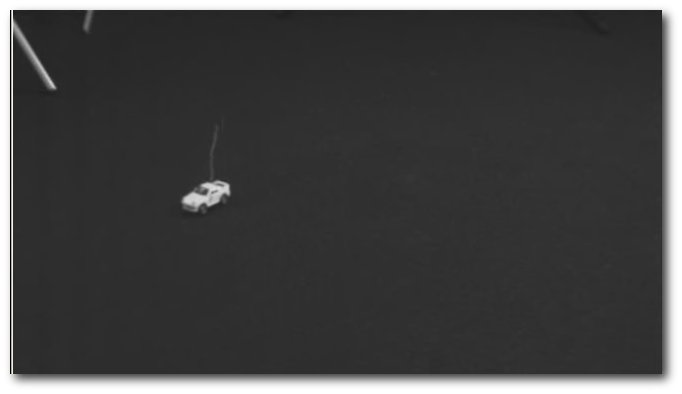
\includegraphics[scale=0.5]{singlecar.jpg}
\caption{\textit{movie12 screenshot}}
\end{figure}

\newpage
\subsubsection{Test 11: MOD=3, Q=1000, S=1000}

\begin{figure}[hb]
\centering
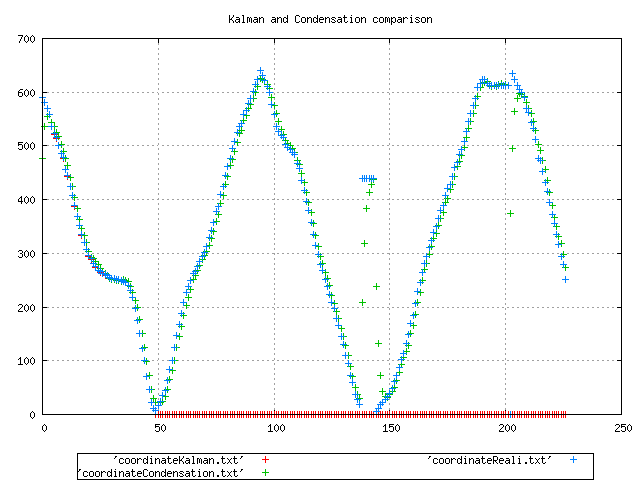
\includegraphics[scale=0.4]{../../esperimenti/single_car/mod_3-Q_1000-S_1000/plot.png}
\caption{\textit{Test 11: Tracciamento}}
\end{figure}

\begin{figure}[hb]
\centering
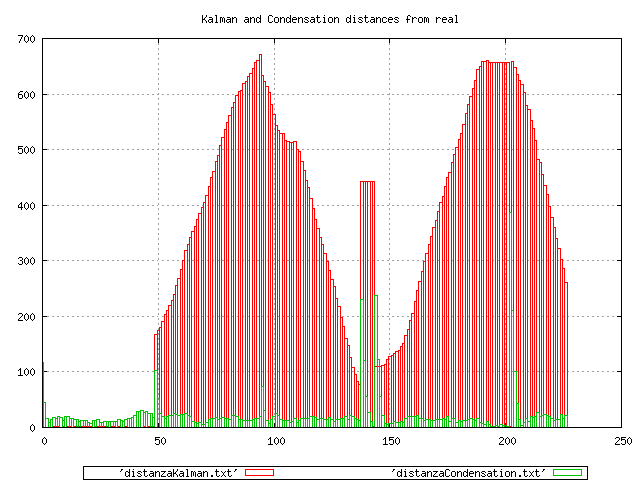
\includegraphics[scale=0.4]{../../esperimenti/single_car/mod_3-Q_1000-S_1000/plot-distances.png}
\caption{\textit{Test 11: Previsioni}}
\end{figure}

Statistiche:
\begin{itemize}
\item \begin{math} \bar \delta_K: 323  \end{math}
\item \begin{math} \bar \delta_C: 23 \end{math}
\item \begin{math}(\sigma_x,\sigma_y)\end{math}: (111,83)
\end{itemize}

In questo test si hanno i risultati più comuni: se l'oggetto scompare dalle scena e riappare in punti molto distanti da dove è scomparso il filtro di Kalman lo perde, ma quando l'oggetto è individuato correttamente Kalman è migliore del Condensation. 
Tuttavia in media il Condensation è molto più preciso nella predizione.

\newpage
\subsubsection{Test 12: MOD=10, Q=5000, S=1000}

\begin{figure}[hb]
\centering
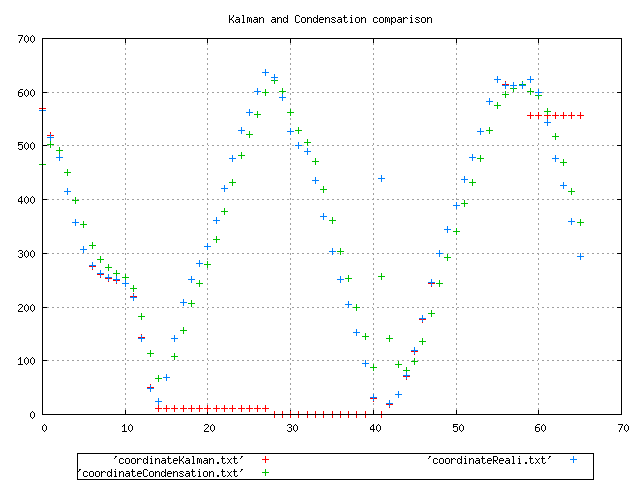
\includegraphics[scale=0.4]{../../esperimenti/single_car/mod_10-Q_5000-S_1000/plot.png}
\caption{\textit{Test 12: Tracciamento}}
\end{figure}

\begin{figure}[hb]
\centering
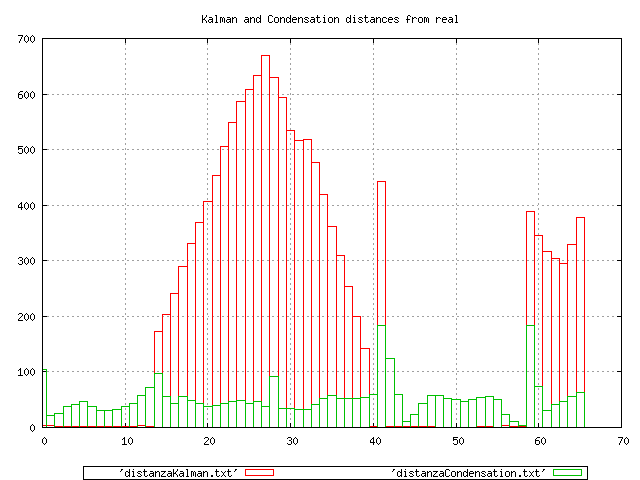
\includegraphics[scale=0.4]{../../esperimenti/single_car/mod_10-Q_5000-S_1000/plot-distances.png}
\caption{\textit{Test 12: Previsioni}}
\end{figure}

Statistiche:
\begin{itemize}
\item \begin{math} \bar \delta_K:  209 \end{math}
\item \begin{math} \bar \delta_C:  52 \end{math}
\item \begin{math}(\sigma_x,\sigma_y)\end{math}: (114,83)
\end{itemize}

Il video in questione si presta ad un tracciamento effettuato ad intervalli anche ampi poichè non ci sono brusche accelerazioni o frenate. Il problema principale sul filtro di Kalman resta che perde l'oggetto se scompare ed è perciò evidente la necessità di incrementare l'area di tolleranza per migliorare le prestazioni del filtro. 

\newpage
\subsubsection{Test 13: MOD=6, Q=1000, S=1000}

\begin{figure}[hb]
\centering
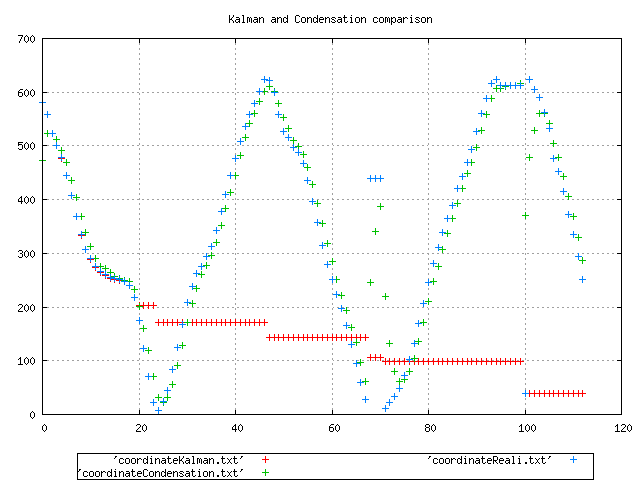
\includegraphics[scale=0.4]{../../esperimenti/single_car/mod_6-Q_1000-S_1000/plot.png}
\caption{\textit{Test 13: Tracciamento}}
\end{figure}

\begin{figure}[hb]
\centering
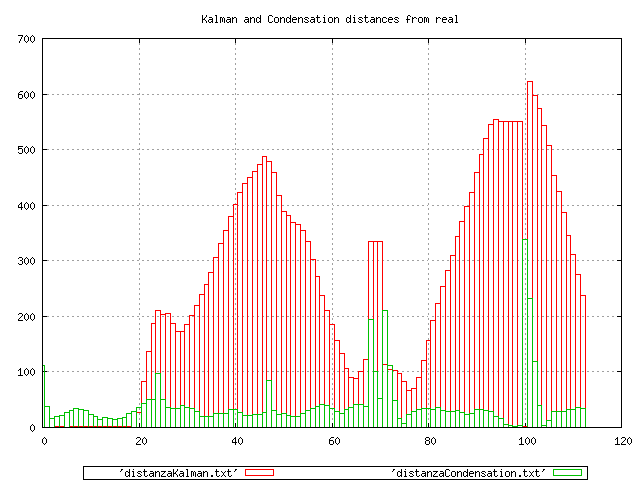
\includegraphics[scale=0.4]{../../esperimenti/single_car/mod_6-Q_1000-S_1000/plot-distances.png}
\caption{\textit{Test 13: Previsioni}}
\end{figure}

Statistiche:
\begin{itemize}
\item \begin{math} \bar \delta_K: 252 \end{math}
\item \begin{math} \bar \delta_C: 40 \end{math}
\item \begin{math}(\sigma_x,\sigma_y)\end{math}: (113,82)
\end{itemize}

Anche riducendo in numero di frames di campionamento la situazione non cambia molto, anzi per un caso crediamo dovuto alla natura del video stesso la situazione addirittura peggiora per il filtro di Kalman.
Decidiamo perciò di togliere il controllo sulla correttezza del rilevamento da parte di Kalman e ci poniamo come unico obiettivo quello di farlo lavorare in condizioni di minima tolleranza sull'errore.

\newpage
\subsubsection{Test 14: MOD=6, Q=1, S=1000}

\begin{figure}[hb]
\centering
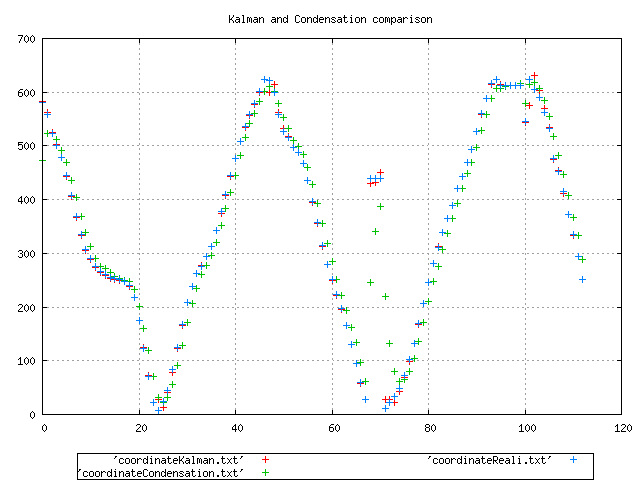
\includegraphics[scale=0.4]{../../esperimenti/single_car/mod_6-Q_1-S_1000/plot.png}
\caption{\textit{Test 14: Tracciamento}}
\end{figure}

\begin{figure}[hb]
\centering
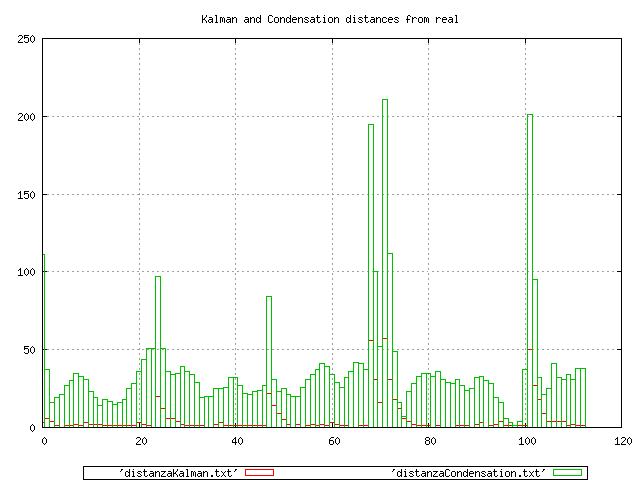
\includegraphics[scale=0.4]{../../esperimenti/single_car/mod_6-Q_1-S_1000/plot-distances.png}
\caption{\textit{Test 14: Previsioni}}
\end{figure}

Statistiche:
\begin{itemize}
\item \begin{math} \bar \delta_K: 5 \end{math}
\item \begin{math} \bar \delta_C: 37 \end{math}
\item \begin{math}(\sigma_x,\sigma_y)\end{math}: (113,82)
\end{itemize}

Togliendo il controllo sulla correttezza della predizione da parte di Kalman, se l'oggetto scompare siamo comuque in grado di tracciarlo (il filtro di Kalman lo ``insegue''). In media Kalman sbaglia pochissimo, il tracciamento è quasi perfetto.
L'obiettivo è ora quello di metterci in una situazione ipotetica in cui Kalman si comporta peggio del Condensation.

\newpage
\subsubsection{Test 15: MOD=6, Q=0.1, S=1000}

\begin{figure}[hb]
\centering
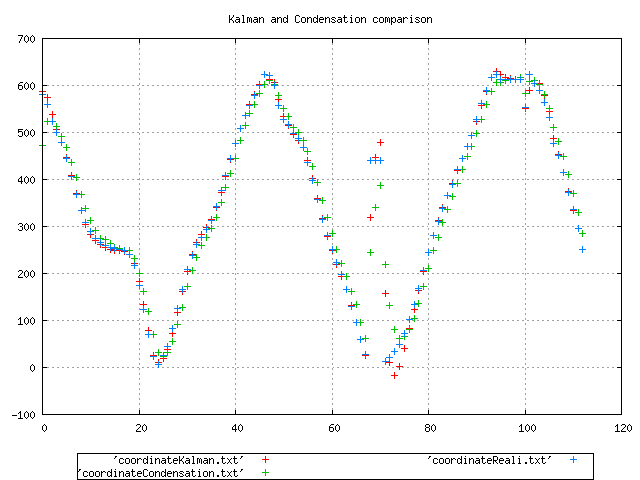
\includegraphics[scale=0.4]{../../esperimenti/single_car/mod_6-Q_0.1-S_1000/plot.png}
\caption{\textit{Test 15: Tracciamento}}
\end{figure}

\begin{figure}[hb]
\centering
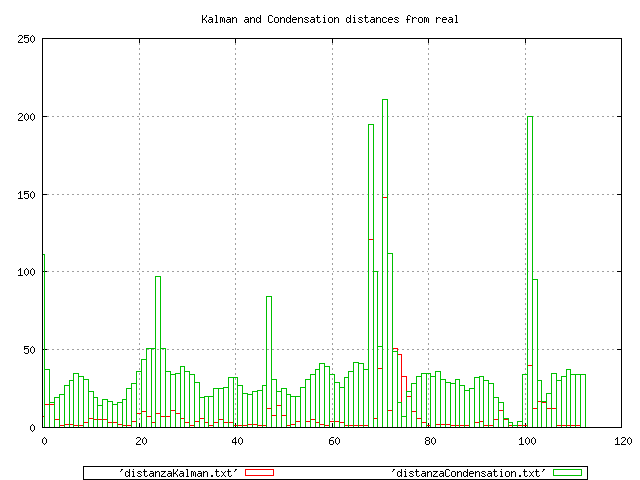
\includegraphics[scale=0.4]{../../esperimenti/single_car/mod_6-Q_0.1-S_1000/plot-distances.png}
\caption{\textit{Test 15: Previsioni}}
\end{figure}

Statistiche:
\begin{itemize}
\item \begin{math} \bar \delta_K: 8 \end{math}
\item \begin{math} \bar \delta_C: 37 \end{math}
\item \begin{math}(\sigma_x,\sigma_y)\end{math}: (113,82)
\end{itemize}

Riduciamo l'errore consentito sulla predizione, l'ellisse di tolleranza si riduce imponendo a Kalma di sbagliare il meno possibile. In questo test i risultati ottenuti non si discostano molto da quelli precedenti, l'oggetto è sempre tracciato ottimamente dal filtro di Kalman.

\newpage
\subsubsection{Test 16: MOD=6, Q=0.001, S=1000}

\begin{figure}[hb]
\centering
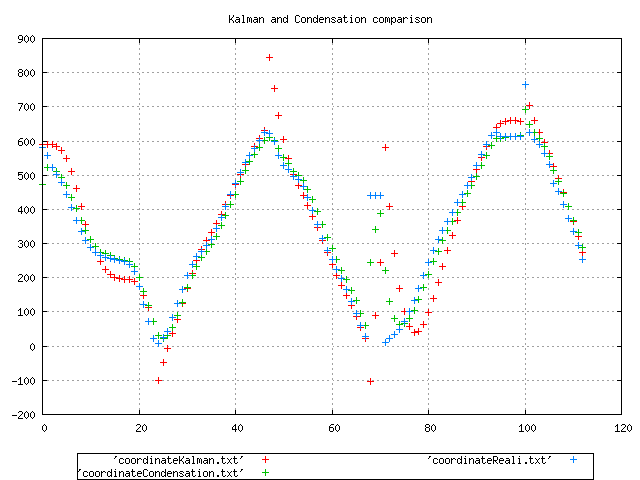
\includegraphics[scale=0.4]{../../esperimenti/single_car/mod_6-Q_0.001-S_1000/plot.png}
\caption{\textit{Test 16: Tracciamento}}
\end{figure}

\begin{figure}[hb]
\centering
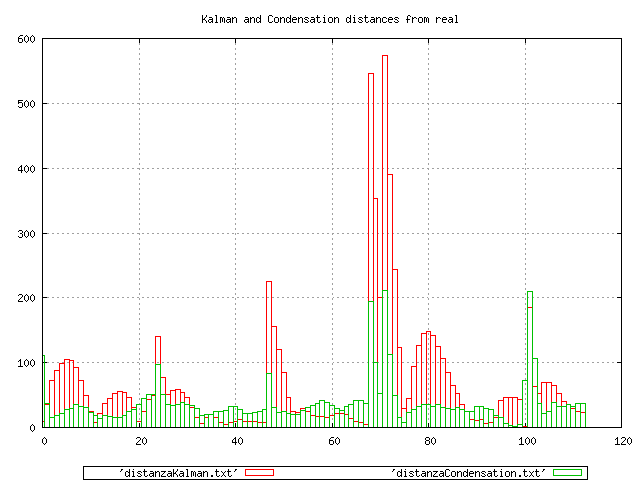
\includegraphics[scale=0.4]{../../esperimenti/single_car/mod_6-Q_0.001-S_1000/plot-distances.png}
\caption{\textit{Test 16: Previsioni}}
\end{figure}

Statistiche:
\begin{itemize}
\item \begin{math} \bar \delta_K: 66 \end{math}
\item \begin{math} \bar \delta_C: 43 \end{math}
\item \begin{math}(\sigma_x,\sigma_y)\end{math}: (114,82)
\end{itemize}

Come previsto il filtro di Kalman comincia finalmente a peggiorare il proprio comportamento anche se in media è sempre migliore dell'altro. 

\newpage
\subsubsection{Test 17: MOD=6, Q=0.0001, S=1000}

\begin{figure}[hb]
\centering
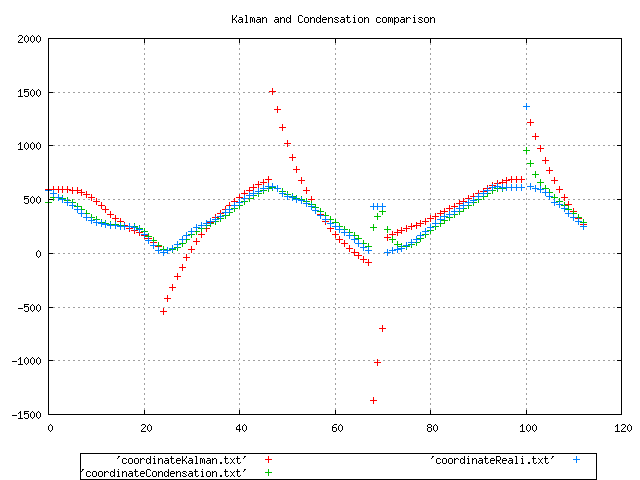
\includegraphics[scale=0.4]{../../esperimenti/single_car/mod_6-Q_0.0001-S_1000/plot.png}
\caption{\textit{Test 17: Tracciamento}}
\end{figure}

\begin{figure}[hb]
\centering
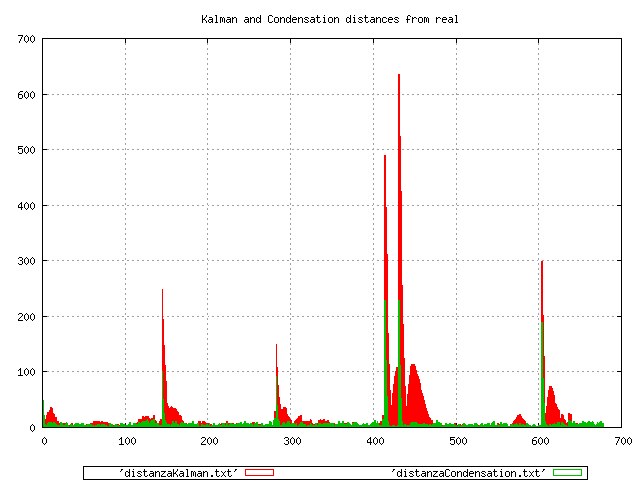
\includegraphics[scale=0.4]{../../esperimenti/single_car/mod_1-Q_0.0001-S_1000/plot-distances.png}
\caption{\textit{Test 17: Previsioni}}
\end{figure}

Statistiche:
\begin{itemize}
\item \begin{math} \bar \delta_K: 179 \end{math}
\item \begin{math} \bar \delta_C: 43 \end{math}
\item \begin{math}(\sigma_x,\sigma_y)\end{math}: (114,83)
\end{itemize}

In questo test Kalman non riesce più a tracciare correttamente l'oggetto. Appare qui evidente come alcune zone si dimostrino particolarmente critiche per il filtro di Kalman.

\newpage
\subsubsection{Test 18: MOD=1, Q=0.0001, S=1000}

\begin{figure}[hb]
\centering
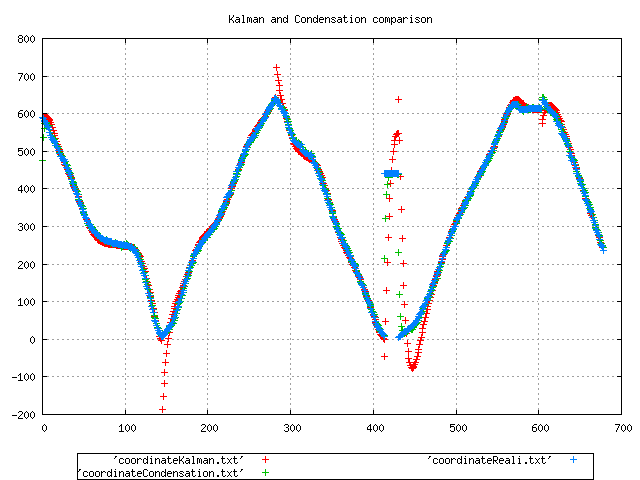
\includegraphics[scale=0.4]{../../esperimenti/single_car/mod_1-Q_0.0001-S_1000/plot.png}
\caption{\textit{Test 18: Tracciamento}}
\end{figure}

\begin{figure}[hb]
\centering
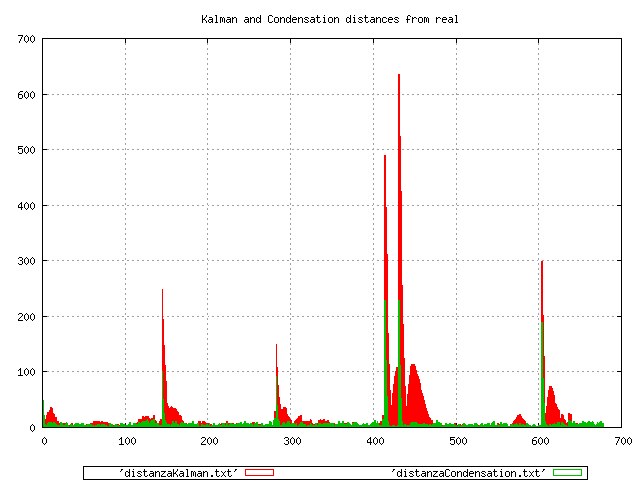
\includegraphics[scale=0.4]{../../esperimenti/single_car/mod_1-Q_0.0001-S_1000/plot-distances.png}
\caption{\textit{Test 18: Previsioni}}
\end{figure}

Abbiamo variato anche la frequenza di campionamento.
Qui il comportamento di Kalman è migliore rispetto al test precedente ed è più chiaro come Kalman si trovi in difficoltà soprattutto nel tracciare zone di non linearità del moto dell'oggetto. (smoothness)

Statistiche:
\begin{itemize}
\item \begin{math} \bar \delta_K: 22 \end{math}
\item \begin{math} \bar \delta_C: 8\end{math}
\item \begin{math}(\sigma_x,\sigma_y)\end{math}: (111,85)
\end{itemize}

